% AI Engineering: Field Notes
% One chapter ("level") per project. Add a new \input line for each project.
%
% Build (from the ai-engineering folder):
%   pdflatex -output-directory=notes/latex/build notes/latex/main.tex   (run twice for the contents page)

\documentclass[11pt,a4paper]{report}

\usepackage[a4paper,margin=20mm]{geometry}
\usepackage[T1]{fontenc}
\usepackage{lmodern}
\renewcommand{\familydefault}{\sfdefault}
\usepackage[varqu,scaled=0.92]{zi4}
\usepackage{amsmath,amssymb}
\usepackage{xcolor}
\usepackage{pifont}
\usepackage{booktabs,array,tabularx}
\usepackage{enumitem}
\usepackage{parskip}
\usepackage{tikz}
\usetikzlibrary{arrows.meta,positioning,calc,decorations.pathreplacing,fit}
\usepackage{pgfplots}
\pgfplotsset{compat=1.18}
\usepackage{listings}
\usepackage[most]{tcolorbox}
\tcbuselibrary{listings}
\usepackage{titlesec}

% ---------- palette ----------
\definecolor{ink}{HTML}{1F2328}
\definecolor{cblue}{HTML}{2B7BB9}
\definecolor{cgold}{HTML}{D98E04}
\definecolor{cgreen}{HTML}{2E8B57}
\definecolor{cred}{HTML}{D64545}
\definecolor{cteal}{HTML}{138A7E}
\definecolor{cpurple}{HTML}{7B5CC4}
\definecolor{cpink}{HTML}{C2409E}
\definecolor{cgray}{HTML}{6B7280}
\definecolor{codebg}{HTML}{F6F8FA}

\usepackage[colorlinks=true,linkcolor=cblue,urlcolor=cblue]{hyperref}

\color{ink}

% ---------- small helpers ----------
\newcommand{\twodigit}[1]{\ifnum#1<10 0\fi#1}
\newcommand{\badge}[2]{\tikz[baseline=(b.base)]\node[fill=#1,text=white,rounded corners=2pt,inner sep=2.2pt,font=\scriptsize\sffamily\bfseries](b){#2};}
\newcommand{\cbadge}[2]{\tikz[baseline=(b.base)]\node[draw=#1,fill=#1!10,text=ink,rounded corners=2pt,inner sep=2.2pt,font=\small\ttfamily](b){#2};}
\newcommand{\xp}[1]{\par\noindent\hfill\badge{cgold}{+#1 XP}\par}
\newcommand{\cmark}{\textcolor{cgreen}{\ding{51}}}
\newcommand{\xmark}{\textcolor{cred}{\ding{55}}}
\newcommand{\warnicon}{\tikz[baseline=-0.6ex]{\fill[cgold] (0,-0.09)--(0.3,-0.09)--(0.15,0.2)--cycle;\node[text=white,font=\tiny\bfseries,inner sep=0] at (0.15,0.025){!};}}
\newcommand{\code}[1]{\texttt{#1}}

% ---------- callout boxes ----------
\tcbset{callout/.style={enhanced,breakable,colback=#1!5,colframe=#1,boxrule=0pt,leftrule=3pt,
  arc=0pt,outer arc=0pt,left=3mm,right=3mm,top=1mm,bottom=1.5mm,
  fonttitle=\sffamily\bfseries\footnotesize,coltitle=#1,colbacktitle=#1!5,titlerule=0pt,
  toptitle=1.5mm,bottomtitle=-0.5mm,before skip=3mm,after skip=3mm}}
\newtcolorbox{keyidea}[1][]{callout=cblue,title={\ding{72}\ \ KEY IDEA#1}}
\newtcolorbox{trap}[1][]{callout=cgold,title={\warnicon\ \ TRAP CARD#1}}
\newtcolorbox{boss}[1][]{callout=cred,title={\ding{110}\ \ BOSS FIGHT#1}}
\newtcolorbox{lab}[1][]{callout=cgreen,title={\ding{115}\ \ LAB RESULT\quad\textmd{measured, not guessed}#1}}
\newtcolorbox{gamerule}[1][]{callout=cteal,title={\ding{228}\ \ RULE#1}}
\newtcolorbox{achievement}[1]{callout=cpurple,title={\ding{72}\ \ ACHIEVEMENT UNLOCKED: #1}}

% ---------- code ----------
\lstdefinestyle{py}{language=Python,basicstyle=\ttfamily\small,keywordstyle=\color{cpurple}\bfseries,
  stringstyle=\color{cgreen!80!black},commentstyle=\color{cgray}\itshape,showstringspaces=false,
  columns=fullflexible,keepspaces=true,upquote=true,breaklines=true}
\newtcblisting{pycode}{listing only,listing options={style=py},enhanced,colback=codebg,
  colframe=cgray!35,boxrule=0.4pt,arc=2pt,left=2mm,right=2mm,top=0.5mm,bottom=0.5mm,
  before skip=2mm,after skip=3mm}
\newtcblisting{rawcode}{listing only,listing options={basicstyle=\ttfamily\footnotesize,
  columns=fullflexible,keepspaces=true,breaklines=true,upquote=true},enhanced,colback=codebg,
  colframe=cgray!35,boxrule=0.4pt,arc=2pt,left=2mm,right=2mm,top=0.5mm,bottom=0.5mm,
  before skip=2mm,after skip=3mm}

% ---------- headings ----------
\titleformat{\chapter}[display]{\sffamily\bfseries\color{ink}}
  {\badge{cgold}{\large LEVEL \twodigit{\thechapter}}}{6pt}{\Huge}
\titleformat{name=\chapter,numberless}[display]{\sffamily\bfseries\color{ink}}{}{0pt}{\Huge}
\titlespacing*{\chapter}{0pt}{0pt}{14pt}
\titleformat{\section}{\sffamily\Large\bfseries\color{ink}}{\textcolor{cgold}{\thesection}}{0.6em}{}
\titleformat{\subsection}{\sffamily\large\bfseries\color{cgray}}{}{0em}{}
\setcounter{secnumdepth}{1}

\begin{document}

% ================= title page =================
\begin{titlepage}
\centering
\vspace*{8mm}
{\sffamily\bfseries\fontsize{38}{42}\selectfont AI ENGINEERING}\\[3mm]
{\Large\sffamily\color{cgray} Field Notes \,\textperiodcentered\, a project-based quest log}\\[14mm]

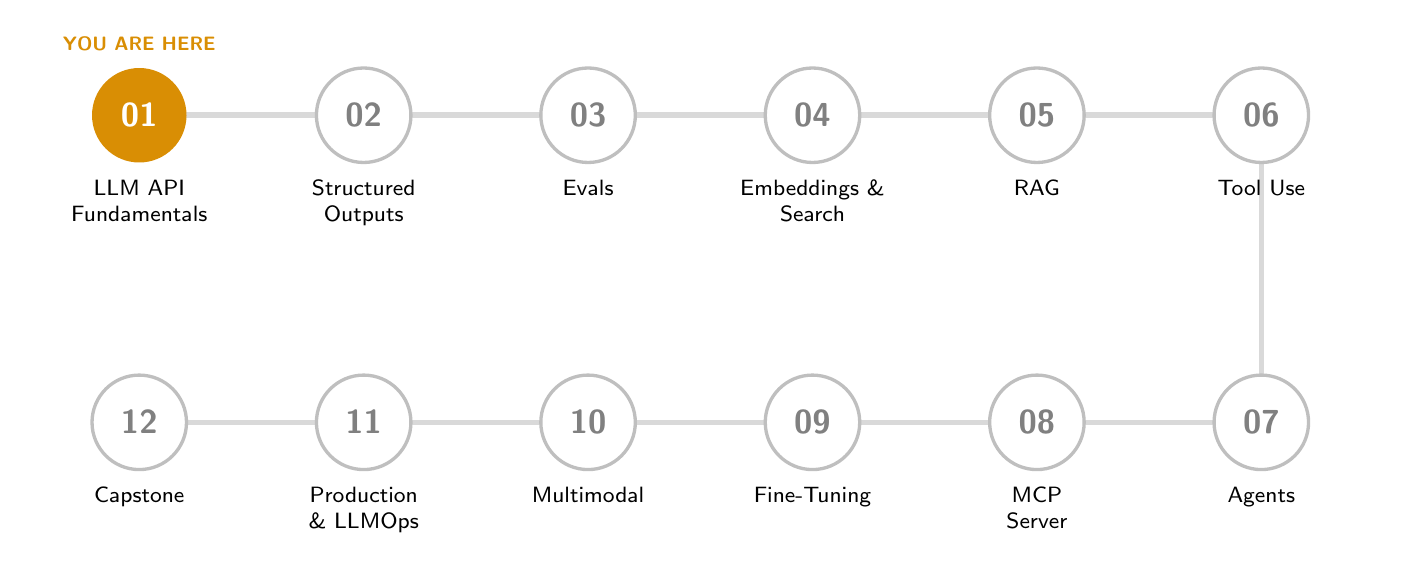
\begin{tikzpicture}
  \foreach \i in {1,...,12} {
    \pgfmathtruncatemacro\row{(\i-1)/6}
    \pgfmathtruncatemacro\col{\row==0 ? \i-1 : 12-\i}
    \coordinate (L\i) at (\col*2.85, -\row*3.9);
  }
  \draw[line width=2pt,gray!30] (L1)--(L2)--(L3)--(L4)--(L5)--(L6)--(L7)--(L8)--(L9)--(L10)--(L11)--(L12);
  \foreach \i/\name in {
      1/LLM API\\Fundamentals, 2/Structured\\Outputs, 3/Evals, 4/Embeddings \&\\Search,
      5/RAG, 6/Tool Use, 7/Agents, 8/MCP\\Server, 9/Fine-Tuning, 10/Multimodal,
      11/Production\\\& LLMOps, 12/Capstone} {
    \ifnum\i=1
      \node[circle,minimum size=12mm,fill=cgold,text=white,font=\sffamily\bfseries\large] at (L\i) {\twodigit{\i}};
    \else
      \node[circle,minimum size=12mm,draw=gray!50,line width=1.2pt,fill=white,text=gray,font=\sffamily\bfseries\large] at (L\i) {\twodigit{\i}};
    \fi
    \node[below=7mm,font=\footnotesize\sffamily,align=center,text width=2.6cm] at (L\i) {\name};
  }
  \node[above=7mm,font=\scriptsize\sffamily\bfseries,text=cgold] at (L1) {YOU ARE HERE};
\end{tikzpicture}

\vfill
\begin{tabular}{@{}l l@{}}
  \badge{cblue}{KEY IDEA} & the concept to remember \\[2pt]
  \badge{cteal}{RULE} & how to do it right \\[2pt]
  \badge{cgold}{TRAP CARD} & a mistake that actually happened \\[2pt]
  \badge{cred}{BOSS FIGHT} & the hard part of a level \\[2pt]
  \badge{cgreen}{LAB RESULT} & numbers measured in our own runs \\[2pt]
  \badge{cpurple}{ACHIEVEMENT} & what you can now do \\
\end{tabular}
\vspace*{8mm}
\end{titlepage}

\tableofcontents

% ============================================================
%  LEVEL 01: LLM API Fundamentals
%  Code: 01-llm-api-fundamentals/
% ============================================================
\chapter{LLM API Fundamentals}

\textbf{Mission:} build a command-line chat assistant on the raw API, no frameworks, and understand
exactly what every call costs and returns.

\begin{center}
\begin{tabular}{@{}c l l r@{}}
\toprule
\textbf{Step} & \textbf{Quest} & \textbf{Status} & \textbf{XP} \\
\midrule
1 & The first call                     & \badge{cgreen}{CLEARED} & 50 \\
2 & A chat that remembers              & \badge{cgreen}{CLEARED} & 65 \\
3 & Streaming                          & \badge{cgreen}{CLEARED} & 60 \\
4 & Settings: system prompt, model, effort & \badge{cblue}{NEXT}  & -- \\
5 & Token budget: trim or summarize    & \badge{cgray}{LOCKED} & -- \\
6 & Errors and retries                 & \badge{cgray}{LOCKED} & -- \\
\bottomrule
\end{tabular}
\end{center}

\begin{tcolorbox}[enhanced,colback=cteal!5,colframe=cteal,boxrule=0.6pt,arc=2pt,
  title={\sffamily\bfseries EQUIPPED MODEL},coltitle=white,colbacktitle=cteal]
\code{claude-haiku-5-5}\quad \$0.10 per 1M input tokens \textperiodcentered{} \$0.50 per 1M output tokens
(prompts up to 100K tokens; above that \$0.50 / \$2.50).\\
Step 1 was first run on \code{claude-opus-5-5} (\$4 / \$20). We switched because a learning project
does not need the biggest model.
\end{tcolorbox}

% ------------------------------------------------------------
\section{Step 1: The first call}
\xp{50}

\subsection{Anatomy of a request}

Every call to a model is one HTTPS request to one endpoint. It has three required parts.

\begin{center}
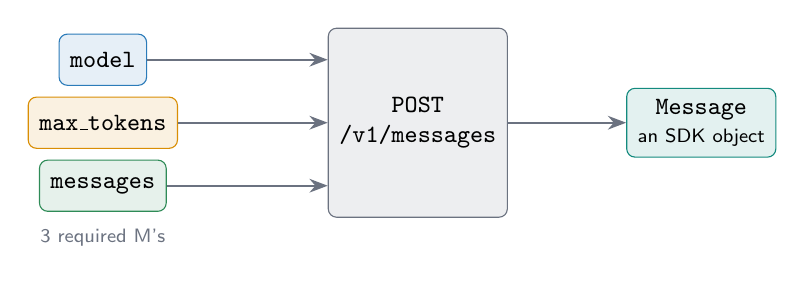
\begin{tikzpicture}[chip/.style={draw=#1,fill=#1!12,rounded corners=3pt,font=\ttfamily\small,
    inner sep=4pt,minimum height=6.5mm},>=Stealth]
  \node[chip=cblue]  (model) at (0,1.0)  {model};
  \node[chip=cgold]  (max)   at (0,0.2)  {max\_tokens};
  \node[chip=cgreen] (msgs)  at (0,-0.6) {messages};
  \node[chip=cgray,minimum height=2.4cm,align=center] (api) at (4,0.2) {POST\\/v1/messages};
  \node[chip=cteal,align=center] (resp) at (7.6,0.2) {Message\\[-1pt]{\scriptsize\sffamily an SDK object}};
  \foreach \n in {model,max,msgs} \draw[->,thick,cgray] (\n.east) -- (api.west |- \n.east);
  \draw[->,thick,cgray] (api) -- (resp);
  \node[font=\scriptsize\sffamily,text=cgray,below=1mm of msgs] {3 required M's};
\end{tikzpicture}
\end{center}

\begin{pycode}
response = client.messages.create(
    model="claude-haiku-5-5",   # which model answers
    max_tokens=4000,            # hard cap on the reply (thinking + text)
    messages=[{"role": "user", "content": "Explain what a token is in 2 sentences"}],
)
\end{pycode}

\begin{keyidea}[: the model is stateless]
Each call starts from zero. The model remembers nothing between calls. Anything it should know
(the whole conversation so far) has to be inside \emph{this} request.
\end{keyidea}

\subsection{Anatomy of a response}

\begin{center}
\begin{tabularx}{\linewidth}{@{}l l X@{}}
\toprule
\textbf{Field} & \textbf{Type} & \textbf{Meaning} \\
\midrule
\code{.content} & \code{list[ContentBlock]} & the reply, as a list of blocks: \code{thinking}, then \code{text} \\
\code{.stop\_reason} & \code{str} & why the model stopped generating \\
\code{.usage.input\_tokens} & \code{int} & everything you sent: system prompt + full history + overhead \\
\code{.usage.output\_tokens} & \code{int} & everything generated, \textbf{including hidden thinking} \\
\bottomrule
\end{tabularx}
\end{center}

\begin{pycode}
for block in response.content:
    if block.type == "text":        # never assume content[0] is the text
        print(block.text)
\end{pycode}

\begin{trap}
\code{content[0]} is not always the text. Opus 5.5 returned a \code{thinking} block first; Haiku 5.5
skipped thinking on the same easy question and returned only \code{text}. Current models decide for
themselves how much to think, so loop and check \code{block.type}.
\end{trap}

\subsection{Tokens are money}

A \textbf{token} is the unit a model reads, writes and bills: roughly $\tfrac34$ of a word.
\emph{unbelievable} might become \cbadge{cblue}{un}\cbadge{cgold}{believ}\cbadge{cgreen}{able}.
An 8-word prompt cost 22 input tokens, because the message wrapper adds overhead.

\[
\text{cost} \;=\; \frac{\text{input tokens}}{10^6}\times p_{\text{in}}
\;+\; \frac{\text{output tokens}}{10^6}\times p_{\text{out}}
\]

Output tokens cost $5\times$ input tokens on both models, and thinking counts as output.

\begin{lab}
Same question (\emph{Explain what a token is in 2 sentences}), one run each:
\begin{center}
\begin{tabular}{@{}l r r r@{}}
\toprule
Model & in & out & cost \\
\midrule
\code{claude-opus-5-5}  & 22 & 142 & \$0.002928 \\
\code{claude-haiku-5-5} & 22 & 73  & \$0.000039 \\
\bottomrule
\end{tabular}
\end{center}
Haiku was $75\times$ cheaper: $40\times$ from the price, the rest because it skipped thinking.
A second Opus run of the same question used 168 output tokens instead of 142:
\textbf{same prompt $\neq$ same output}, so measure more than one run.
\end{lab}

\subsection{The \texttt{max\_tokens} boss}

\begin{center}
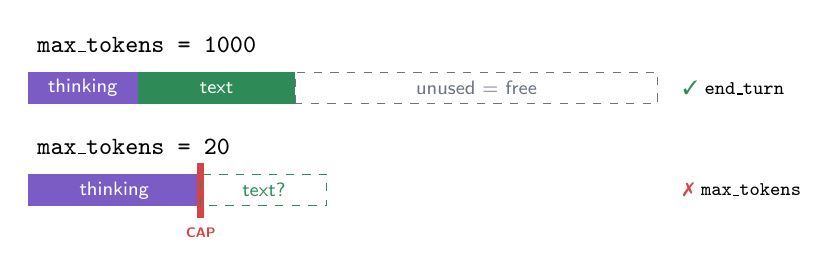
\begin{tikzpicture}[x=1cm,y=1cm,font=\sffamily\scriptsize]
  % run 1
  \node[anchor=west,font=\ttfamily\small] at (0,2.35) {max\_tokens = 1000};
  \fill[cpurple] (0,1.6) rectangle (1.4,2.0);   \node[text=white] at (0.7,1.8) {thinking};
  \fill[cgreen]  (1.4,1.6) rectangle (3.4,2.0); \node[text=white] at (2.4,1.8) {text};
  \draw[cgray,dashed] (3.4,1.6) rectangle (8,2.0); \node[text=cgray] at (5.7,1.8) {unused = free};
  \node[anchor=west] at (8.2,1.8) {\cmark\ \code{end\_turn}};
  % run 2
  \node[anchor=west,font=\ttfamily\small] at (0,1.05) {max\_tokens = 20};
  \fill[cpurple] (0,0.3) rectangle (2.2,0.7); \node[text=white] at (1.1,0.5) {thinking};
  \draw[cred,line width=2.5pt] (2.2,0.15) -- (2.2,0.85); \node[text=cred,font=\sffamily\bfseries\tiny,below] at (2.2,0.15) {CAP};
  \draw[cgreen,dashed] (2.2,0.3) rectangle (3.8,0.7); \node[text=cgreen] at (3.0,0.5) {text?};
  \node[anchor=west] at (8.2,0.5) {\xmark\ \code{max\_tokens}};
\end{tikzpicture}
\end{center}

\begin{boss}[: thinking ate the whole budget]
With \code{max\_tokens=20} on Opus, \code{stop\_reason} was \code{max\_tokens} and there was
\textbf{no text at all}: thinking used all 20 tokens before the answer started. We were still billed
for 20 output tokens.\\[2pt]
\textbf{Strategy:} \code{max\_tokens} is a ceiling, not a target, and unused tokens are free. Set it
generously (4000) and always check \code{stop\_reason}.
\end{boss}

\subsection{\texttt{stop\_reason}: status effects}

\begin{center}
\begin{tabular}{@{}l l@{}}
\cbadge{cgreen}{end\_turn} & finished normally: safe to use \\[2pt]
\cbadge{cred}{max\_tokens} & hit your cap: the answer is incomplete (or missing) \\[2pt]
\cbadge{cgold}{tool\_use} & wants \emph{you} to run a tool (Level 06) \\[2pt]
\cbadge{cgray}{refusal} & the model declined the request \\[2pt]
\cbadge{cpink}{model\_context\_window\_exceeded} & the history no longer fits the model (Step 5) \\
\end{tabular}
\end{center}

\begin{gamerule}
Check \code{stop\_reason} \textbf{before} trusting \code{content}. It is a plain \code{str}, so compare
with \code{==}.
\end{gamerule}

\begin{trap}
API keys never go in code. Ours lives in a Windows user environment variable; a \code{.env} file
(listed in \code{.gitignore}) also works. \code{anthropic.Anthropic()} finds it by itself.
\end{trap}

\begin{achievement}{First Call \textperiodcentered{} Priced a Call \textperiodcentered{} Beat the Boss}
You can make a call, read every part of the response, and say what it cost.
\end{achievement}

% ------------------------------------------------------------
\section{Step 2: A chat that remembers}
\xp{65}

\begin{keyidea}[: memory is a list you resend]
A chat app fakes memory. It keeps the whole conversation in a list and sends \textbf{all of it} with
every call. Forget to append the assistant's reply and the model never sees what it said before.
\end{keyidea}

\begin{center}
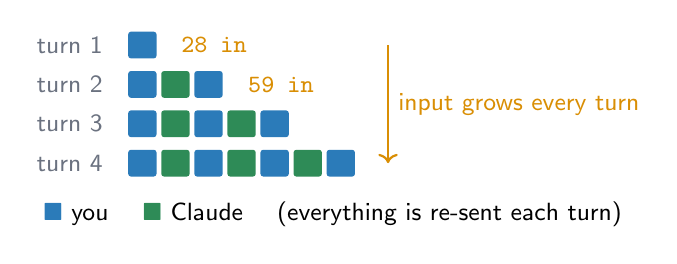
\begin{tikzpicture}[x=1cm,y=1cm]
  \foreach \row in {1,2,3,4} {
    \node[anchor=east,font=\sffamily\small,text=cgray] at (-0.2,-\row*0.5) {turn \row};
    \pgfmathtruncatemacro\nblk{2*\row-1}
    \foreach \idx in {1,...,\nblk} {
      \ifodd\idx\relax\def\blkcol{cblue}\else\def\blkcol{cgreen}\fi
      \fill[fill=\blkcol,rounded corners=1pt] ({(\idx-1)*0.42},{-\row*0.5-0.17}) rectangle ++(0.36,0.34);
    }
  }
  \node[anchor=west,font=\ttfamily\small,text=cgold] at (0.55,-0.5) {28 in};
  \node[anchor=west,font=\ttfamily\small,text=cgold] at (1.4,-1.0) {59 in};
  \draw[->,thick,cgold] (3.3,-0.5) -- (3.3,-2.0) node[midway,right,font=\sffamily\small] {input grows every turn};
  \node[anchor=west,font=\sffamily\small] at (-1.2,-2.65)
    {\textcolor{cblue}{$\blacksquare$} you \quad \textcolor{cgreen}{$\blacksquare$} Claude \quad (everything is re-sent each turn)};
\end{tikzpicture}
\end{center}

\begin{pycode}
messages = []                                   # the whole session lives here
while True:
    user_text = input("You: ").strip()
    if user_text.lower() in ["quit", "exit"]:
        break
    messages.append({"role": "user", "content": user_text})
    response = client.messages.create(model=MODEL, max_tokens=MAX_TOKENS, messages=messages)
    messages.append({"role": "assistant", "content": response.content})   # ALL blocks
\end{pycode}

\begin{gamerule}
Append \code{response.content} (all blocks, thinking included), not just the text. The API expects
thinking blocks to come back unchanged.
\end{gamerule}

\begin{lab}
Turn 1: \emph{My name is Sam} $\to$ 28 input tokens. Turn 2: \emph{What is my name?} $\to$ 59 input
tokens, and it answered \emph{Sam}. Sending only the latest message instead of the list: it forgot the
name, and input tokens dropped back down.
\end{lab}

\subsection{How the cost grows}

If each exchange adds about $k$ tokens, turn $n$ re-sends about $n\cdot k$ tokens. So:
\[
\text{cost of turn } n \;\propto\; n \quad\text{(linear)}
\qquad\qquad
\text{session total after } n \text{ turns} \;\propto\; \frac{n(n+1)}{2} \quad\text{(quadratic)}
\]

\begin{center}
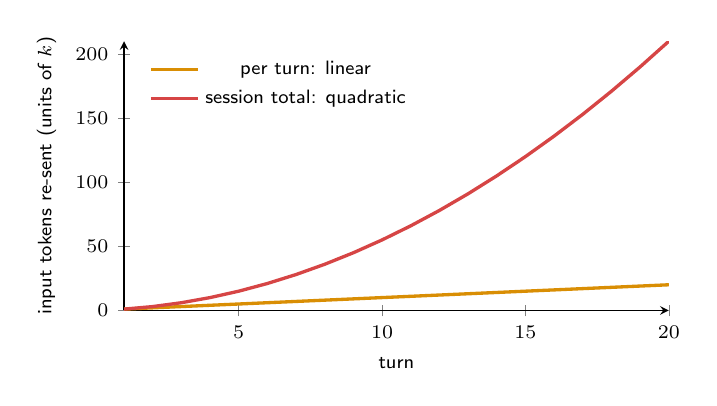
\begin{tikzpicture}
\begin{axis}[width=8.5cm,height=5cm,xlabel={turn},ylabel={input tokens re-sent (units of $k$)},
  axis lines=left,legend style={draw=none,font=\scriptsize\sffamily,at={(0.03,0.97)},anchor=north west},
  tick label style={font=\scriptsize},label style={font=\scriptsize\sffamily},ymin=0]
  \addplot[cgold,very thick,domain=1:20,samples=20] {x};
  \addlegendentry{per turn: linear}
  \addplot[cred,very thick,domain=1:20,samples=20] {x*(x+1)/2};
  \addlegendentry{session total: quadratic}
\end{axis}
\end{tikzpicture}
\end{center}

\begin{trap}
The first thing that breaks is not the context window (1M tokens on Haiku 5.5) but the
\textbf{price}. Once one request is over 100K tokens, Haiku charges \$0.50 / \$2.50 per 1M instead of
\$0.10 / \$0.50. Eventually \code{stop\_reason} becomes \code{model\_context\_window\_exceeded}. Step 5
fixes this by trimming or summarizing old history.
\end{trap}

\subsection{Sessions}

\textbf{1 run = 1 session = 1 list.} When the script exits, the list is gone; the API stores
nothing. Apps like Claude.ai keep each conversation in a database and resend it. To make a session
survive a restart, save the list to JSON (see the next section for why \code{model\_dump()} is needed).

\begin{trap}
\code{"\textbackslash\$"} inside a Python string is not an escape: it prints a literal backslash and raises a
\code{SyntaxWarning}. Just write \code{\$}.
\end{trap}

\begin{achievement}{Gave Claude a Memory}
You can build a multi-turn chat and explain why long chats get expensive.
\end{achievement}

% ------------------------------------------------------------
\section{Types: dicts in, objects out}

\begin{keyidea}
\textbf{You send plain dicts. You get SDK objects back.} Mixing them up causes most beginner errors.
\end{keyidea}

\noindent
\begin{minipage}[t]{0.47\linewidth}
\textbf{\textcolor{cgreen}{YOU SEND}} \cbadge{cgreen}{dict}
\begin{pycode}
messages = [
  {"role": "user",
   "content": "My name is Sam"},
  {"role": "assistant",
   "content": response.content},
]
\end{pycode}
\small Read with \textbf{brackets}: \code{msg["role"]}.
\code{MessageParam} is only a type hint for your editor; at runtime it is a plain dict.
\end{minipage}\hfill
\begin{minipage}[t]{0.49\linewidth}
\textbf{\textcolor{cteal}{YOU GET}} \cbadge{cteal}{Message} {\small (a pydantic object)}\par\smallskip
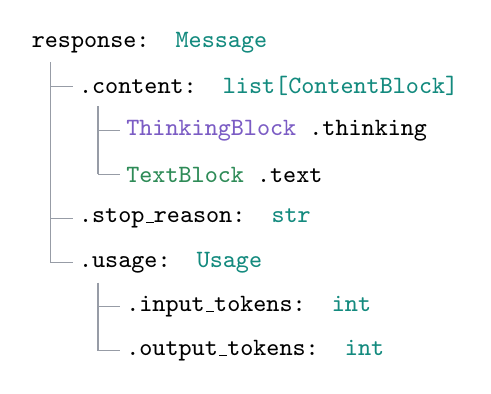
\begin{tikzpicture}[font=\ttfamily\small,every node/.style={anchor=west,inner sep=1.5pt},x=1cm,y=-0.56cm]
  \node at (0,0)   {response: \textcolor{cteal}{Message}};
  \node at (0.6,1) {.content: \textcolor{cteal}{list[ContentBlock]}};
  \node at (1.2,2) {\textcolor{cpurple}{ThinkingBlock}\ .thinking};
  \node at (1.2,3) {\textcolor{cgreen}{TextBlock}\ .text};
  \node at (0.6,4) {.stop\_reason: \textcolor{cteal}{str}};
  \node at (0.6,5) {.usage: \textcolor{cteal}{Usage}};
  \node at (1.2,6) {.input\_tokens: \textcolor{cteal}{int}};
  \node at (1.2,7) {.output\_tokens: \textcolor{cteal}{int}};
  \draw[cgray!70] (0.3,0.45) -- (0.3,5);
  \foreach \y in {1,4,5} \draw[cgray!70] (0.3,\y) -- (0.58,\y);
  \draw[cgray!70] (0.9,1.45) -- (0.9,3);
  \foreach \y in {2,3} \draw[cgray!70] (0.9,\y) -- (1.18,\y);
  \draw[cgray!70] (0.9,5.45) -- (0.9,7);
  \foreach \y in {6,7} \draw[cgray!70] (0.9,\y) -- (1.18,\y);
\end{tikzpicture}\par
\small Read with \textbf{dots}: \code{block.text}. \code{ContentBlock} is a union of block types, so
check \code{block.type} first.
\end{minipage}

\begin{gamerule}[S OF THE GAME]
\begin{itemize}[leftmargin=1.4em,itemsep=4pt]
\item[\cmark] \code{block.text}\par
  {\small\color{cgray} objects are read with dots}
\item[\xmark] \code{block["text"]}\par
  {\small\color{cgray} \code{TypeError: 'TextBlock' object is not subscriptable}}
\item[\cmark] \code{[b.model\_dump() for b in response.content]}\par
  {\small\color{cgray} turns objects into JSON-safe dicts (needed to save a session)}
\item[\xmark] \code{json.dumps(response.content)}\par
  {\small\color{cgray} \code{TypeError: Object of type TextBlock is not JSON serializable}}
\item[\cmark] \code{\{"role": "assistant", "content": response.content\}}\par
  {\small\color{cgray} the SDK accepts its own objects back, so no conversion is needed here}
\end{itemize}
\end{gamerule}

\begin{lab}
Both errors above were reproduced against the installed SDK (\code{anthropic} 2.0.0), not
recalled from memory.
\end{lab}

% ------------------------------------------------------------
\section{API vs SDK}

\begin{center}
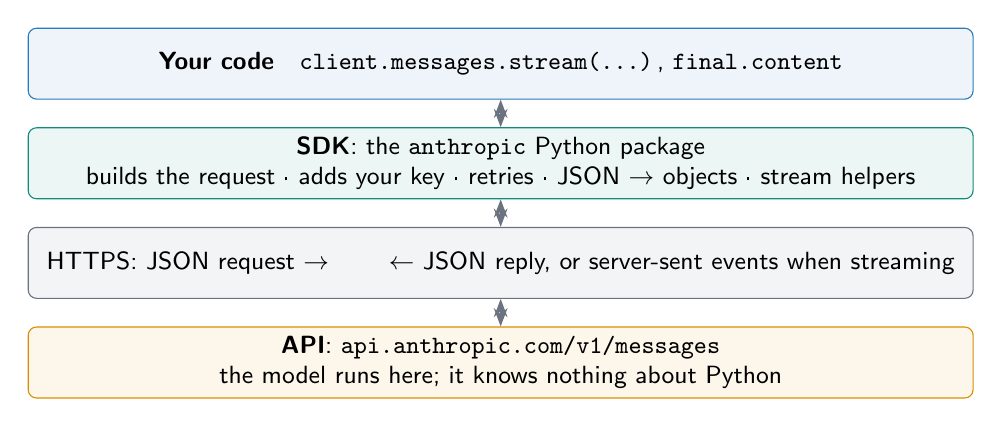
\begin{tikzpicture}[layer/.style={draw=#1,fill=#1!8,rounded corners=3pt,minimum width=12cm,
    minimum height=9mm,align=center,font=\sffamily\small},node distance=3.5mm,>=Stealth]
  \node[layer=cblue] (code) {\textbf{Your code}\quad \code{client.messages.stream(...)}\,, \code{final.content}};
  \node[layer=cteal,below=of code] (sdk) {\textbf{SDK}: the \code{anthropic} Python package\\
    builds the request \textperiodcentered{} adds your key \textperiodcentered{} retries \textperiodcentered{}
    JSON $\to$ objects \textperiodcentered{} stream helpers};
  \node[layer=cgray,below=of sdk] (http) {HTTPS: JSON request $\to$ \qquad $\leftarrow$ JSON reply, or server-sent events when streaming};
  \node[layer=cgold,below=of http] (api) {\textbf{API}: \code{api.anthropic.com/v1/messages}\\
    the model runs here; it knows nothing about Python};
  \draw[<->,thick,cgray] (code) -- (sdk);
  \draw[<->,thick,cgray] (sdk) -- (http);
  \draw[<->,thick,cgray] (http) -- (api);
\end{tikzpicture}
\end{center}

\begin{gamerule}[: the curl test]
\emph{Could I do this with \code{curl}?} \textbf{Yes} $\to$ it is the API: field names
(\code{max\_tokens}, \code{stop\_reason}, \code{usage}) and stream event names.
\textbf{No} $\to$ it is the SDK: Python methods and classes such as \code{get\_final\_message()},
\code{text\_stream}, \code{TextBlock}, \code{model\_dump()}.
\end{gamerule}

\begin{lab}
A raw streaming call with \code{curl} and no Python (shortened):
\begin{rawcode}
event: message_start
data: {"type":"message_start","message":{... "usage":{"input_tokens":17, ...}}}
event: content_block_start
data: {"type":"content_block_start","index":0,"content_block":{"type":"text","text":""}}
event: ping
event: content_block_delta
data: {"type":"content_block_delta","index":0,"delta":{"type":"text_delta","text":"Hello there,"}}
event: content_block_delta
data: {"type":"content_block_delta","index":0,"delta":{"type":"text_delta","text":" friend!"}}
event: content_block_stop
event: message_delta
data: {"type":"message_delta","delta":{"stop_reason":"end_turn"},"usage":{"output_tokens":10, ...}}
event: message_stop
\end{rawcode}
No \code{text}, \code{thinking} or \code{signature} events: those are added by the SDK.
\end{lab}

% ------------------------------------------------------------
\section{Step 3: Streaming}
\xp{60}

\begin{keyidea}[: delivery, not content]
Streaming changes \textbf{how} the answer arrives, not \textbf{what} it is: same model, same
answer quality, same tokens, same cost. The connection stays open and the reply arrives in pieces
(events) while it is being written.
\end{keyidea}

\subsection{One stream = one reply}

\begin{center}
\begin{tabular}{@{}l l l@{}}
\toprule
\textbf{Event} & \textbf{How often} & \textbf{Carries} \\
\midrule
\code{message\_start}       & once            & message id, model, starting usage \\
\quad\code{content\_block\_start} & once per block & which block begins: \code{thinking} or \code{text} \\
\quad\quad\code{content\_block\_delta} & many & the pieces: \code{thinking\_delta}, \code{text\_delta}, \code{signature\_delta} \\
\quad\code{content\_block\_stop}  & once per block & block finished \\
\code{message\_delta}       & once            & \code{stop\_reason} + final usage \\
\code{message\_stop}        & once            & reply finished \\
\bottomrule
\end{tabular}
\end{center}

\begin{trap}
The Python SDK adds extra events named \code{text}, \code{thinking} and \code{signature} that
\emph{repeat} the delta data. Printing both doubles your output. (The raw API also sends
\code{ping} keep-alives.)
\end{trap}

\subsection{TTFT vs total time}

\begin{center}
\begin{tabular}{@{}l l c@{}}
\toprule
\textbf{Metric} & \textbf{Meaning} & \textbf{Streaming helps?} \\
\midrule
TTFT (time to first token) & how long the user stares at nothing & \cmark\ a lot \\
Total time & time until the last word & \xmark\ about the same \\
\bottomrule
\end{tabular}
\end{center}

\begin{center}
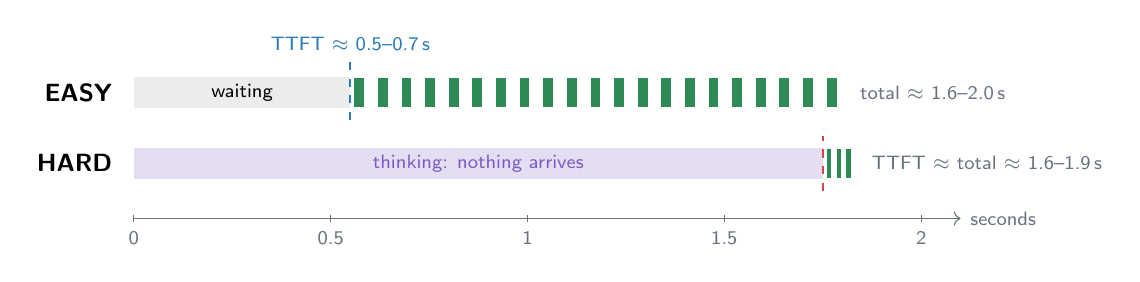
\begin{tikzpicture}[x=5cm,y=1cm,font=\sffamily\scriptsize]
  \draw[->,cgray] (0,0) -- (2.1,0) node[right] {seconds};
  \foreach \t in {0,0.5,1,1.5,2} \draw[cgray] (\t,0.05) -- (\t,-0.05) node[below] {\t};
  % EASY
  \node[anchor=east,font=\sffamily\small\bfseries] at (-0.03,1.6) {EASY};
  \fill[gray!15] (0,1.4) rectangle (0.55,1.8); \node at (0.275,1.6) {waiting};
  \foreach \t in {0.56,0.62,...,1.76} \fill[cgreen] (\t,1.42) rectangle ++(0.025,0.36);
  \draw[cblue,thick,dashed] (0.55,1.25) -- (0.55,2.0) node[above] {TTFT $\approx$ 0.5--0.7\,s};
  \node[anchor=west,text=cgray] at (1.82,1.6) {total $\approx$ 1.6--2.0\,s};
  % HARD
  \node[anchor=east,font=\sffamily\small\bfseries] at (-0.03,0.7) {HARD};
  \fill[cpurple!20] (0,0.5) rectangle (1.75,0.9); \node[text=cpurple] at (0.875,0.7) {thinking: nothing arrives};
  \foreach \t in {1.76,1.785,...,1.83} \fill[cgreen] (\t,0.52) rectangle ++(0.012,0.36);
  \draw[cred,thick,dashed] (1.75,0.35) -- (1.75,1.05);
  \node[anchor=west,text=cgray] at (1.85,0.7) {TTFT $\approx$ total $\approx$ 1.6--1.9\,s};
\end{tikzpicture}
\end{center}

\begin{lab}
Haiku 5.5, two runs each. EASY (\emph{why is the sky blue}) did not think: first text after
0.47--0.67\,s, done after 1.61--1.97\,s. HARD (a marbles puzzle) thought first: nothing arrived for
1.63--1.94\,s, then the thinking summary and the answer came in one burst. A hard question can
triple TTFT.
\end{lab}

\subsection{Streaming inside the chat: two loops}

\begin{pycode}
while True:                                       # OUTER loop: one pass per turn
    ...
    messages.append({"role": "user", "content": user_text})
    print("\nClaude: ", end="", flush=True)
    with client.messages.stream(model=MODEL, max_tokens=MAX_TOKENS,
                                messages=messages) as stream:
        for text in stream.text_stream:           # INNER loop: one pass per piece
            print(text, end="", flush=True)
        final = stream.get_final_message()        # the same Message create() returns
    print()                                       # streamed text never ends in a newline
    messages.append({"role": "assistant", "content": final.content})
\end{pycode}

\begin{lab}
Same question through the step 2 chat and the streaming chat: both \code{29 in / 11 out,
\$0.000008}. Streaming did not change the cost.
\end{lab}

\begin{trap}[: the silent pause]
On a hard question there is a pause after \code{Claude:}. The model is thinking, and two things
hide it: \code{text\_stream} only yields \code{text\_delta} pieces, and thinking text is empty by
default anyway (it only has text with \code{thinking=\{"type": "adaptive", "display": "summarized"\}}).
Those thinking tokens are still billed as output.
\end{trap}

\subsection{Why streaming matters beyond looks}

\begin{itemize}[leftmargin=1.2em,itemsep=2pt]
  \item \textbf{Long requests stay alive.} A non-streaming call sits silent until the end and can time
        out; the SDK refuses non-streaming requests it estimates will take more than about 10 minutes.
        A stream keeps sending data (\code{ping}).
  \item \textbf{You can act early:} a stop button, cancelling halfway, processing the start of the answer.
  \item \textbf{Partial failure is possible:} a dropped connection leaves half an answer.
        \code{get\_final\_message()} assembles the full \code{Message} for you.
\end{itemize}

\begin{achievement}{Read the Stream \textperiodcentered{} Measured TTFT}
You can explain every event in a stream, measure what the user actually waits for, and stream a
multi-turn chat.
\end{achievement}

% ------------------------------------------------------------
\section*{Level 01 progress}
\addcontentsline{toc}{section}{Level 01 progress}

\begin{center}
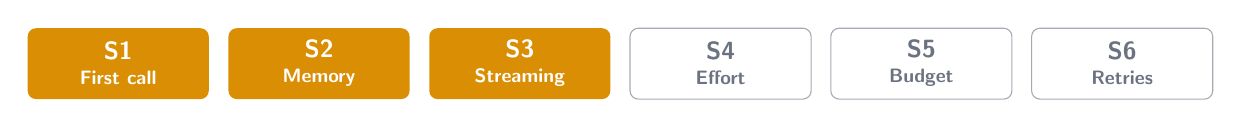
\begin{tikzpicture}
  \foreach \i/\lab/\done in {1/First call/1,2/Memory/1,3/Streaming/1,4/Effort/0,5/Budget/0,6/Retries/0} {
    \ifnum\done=1
      \node[fill=cgold,text=white,rounded corners=3pt,minimum width=2.3cm,minimum height=9mm,
        font=\sffamily\bfseries\small,align=center] at (\i*2.55,0) {S\i\\[-2pt]{\scriptsize\lab}};
    \else
      \node[draw=cgray!60,text=cgray,rounded corners=3pt,minimum width=2.3cm,minimum height=9mm,
        font=\sffamily\bfseries\small,align=center] at (\i*2.55,0) {S\i\\[-2pt]{\scriptsize\lab}};
    \fi
  }
\end{tikzpicture}

\badge{cgold}{175 XP earned}\quad \textbf{Next quest:} Step 4, settings and \emph{effort}
(the replacement for temperature).
\end{center}


\end{document}
